\documentclass[11pt,a4paper]{article}

% Packages
\usepackage[utf8]{inputenc}
\usepackage[english]{babel}
\usepackage{graphicx}
\usepackage{geometry}
\usepackage{hyperref}
\usepackage{longtable}
\usepackage{booktabs}
\usepackage{array}
\usepackage{enumitem}
\usepackage{titlesec}
\usepackage{listings}
\usepackage{xcolor}
\usepackage{float}
\usepackage{ragged2e}
\usepackage{microtype}

% Page geometry
\geometry{a4paper, margin=2.5cm}

% Hyperref setup
\hypersetup{
    colorlinks=true,
    linkcolor=blue,
    filecolor=magenta,
    urlcolor=cyan,
    pdftitle={Smart Audiobook Player Project Report},
    pdfauthor={John Nguyen, Khaled Rami Omar, Jahye Ali},
}

% Title formatting
\titleformat{\section}{\Large\bfseries}{\thesection}{1em}{}
\titleformat{\subsection}{\large\bfseries}{\thesubsection}{1em}{}
\titleformat{\subsubsection}{\normalsize\bfseries}{\thesubsubsection}{1em}{}

% Code listing setup
\lstset{
    basicstyle=\ttfamily\small,
    breaklines=true,
    frame=single,
    backgroundcolor=\color{gray!10}
}

\begin{document}

% Title Page
\begin{titlepage}
    \centering
    \vspace*{2cm}

    {\Huge\bfseries Smart Audiobook Player\par}
    \vspace{0.5cm}
    {\Large Project Report\par}
    \vspace{2cm}

    {\large
    \textbf{Course:} Mobile Application Development\par
    \vspace{0.5cm}
    \textbf{Report Type:} Final Project Rapport\par
    \vspace{1cm}

    \textbf{Group Members:}\par
    \vspace{0.3cm}
    John Nguyen (202209849)\par
    Khaled Rami Omar (202307853)\par
    Jahye Ali (202309135)\par
    \vspace{1cm}

    \textbf{Delivery Date:} 25 March 2026\par
    }

    \vfill
\end{titlepage}

% Table of Contents
\tableofcontents
\clearpage

% Main Content
\section{App Vision and Scope}

Smart Audiobook Player is a premium mobile audiobook app focused on smooth long-form listening, especially for M4B/M4A files.

The app solves common audiobook pain points: poor chapter support, weak resume accuracy, and inconsistent playback across sessions/devices. It offers secure user accounts, cloud-synced progress, chapter-aware playback, and a minimalist high-contrast interface designed for distraction-free listening.

\subsection{Project Scope}

\textbf{In Scope:}
\begin{itemize}[noitemsep]
    \item User authentication with Firebase Authentication (email/password).
    \item Cloud data management using Firestore (progress sync under \texttt{users/\{uid\}/progress/\{bookId\}}).
    \item Core screens: Library, Player, Book Details, and Settings (with integrated profile).
    \item Chapter-aware playback with speed control (0.5x--2.0x), sleep timer, and precise resume.
    \item HTTP API integration (manual REST calls via Retrofit/OkHttp) to enrich metadata from OpenLibrary.
    \item Notification-based playback controls, daily reminders, and engagement notifications.
    \item Biometric library lock with in-app toggle.
\end{itemize}

\textbf{Out of Scope:}
\begin{itemize}[noitemsep]
    \item Multi-platform clients (iOS/Web).
    \item Marketplace/store functionality for buying or downloading books.
    \item Social/community features (reviews, sharing).
\end{itemize}

\section{Technologies}

This section highlights the technology stack as required by the project specification.

\subsection{Mandatory Technologies}

\begin{itemize}[noitemsep]
    \item \textbf{Firebase Authentication:} Email/password sign-in for account-based personalization. Implemented in \texttt{Auth-} \texttt{Repository} with dedicated \texttt{Sign-} \texttt{In-} \texttt{Screen} and \texttt{Sign-} \texttt{Up-} \texttt{Screen} flows integrated into Compose Navigation.
    \item \textbf{Cloud Firestore:} Stores user progress, engagement stats, and FCM tokens under user-scoped paths. Security rules enforce authenticated access: each user can only read/write their own documents. Real-time listeners (\texttt{addSnapshotListener}) enable cross-device sync.
    \item \textbf{External HTTP API (manual calls):} OpenLibrary REST API called via Retrofit/OkHttp for cover art and metadata enrichment when local M4B tags are incomplete. Calls are made directly---no Firebase SDK or wrapper---satisfying the manual HTTP requirement.
\end{itemize}

\subsection{Advanced Technologies (Differentiators)}

\begin{itemize}[noitemsep]
    \item \textbf{Media3 ExoPlayer:} The entire playback engine is built on Jetpack Media3. ExoPlayer handles M4B/M4A decoding, chapter metadata extraction, and seek operations for files that can exceed 20 hours.
    \item \textbf{MediaSession API:} A \texttt{Media-} \texttt{Session-} \texttt{Service} (\texttt{Playback-} \texttt{Service}) decouples playback from the UI process. The UI communicates exclusively through a \texttt{Media-} \texttt{Controller} wrapper (\texttt{Audiobook-} \texttt{Player}), enabling system-level integration with Bluetooth controls, lock screen media controls, and Android Auto.
    \item \textbf{Biometric API:} \texttt{BiometricPrompt} with \texttt{BiometricManager} provides optional library-lock functionality. A settings toggle persists the preference via DataStore, and \texttt{MainActivity} enforces the lock on app launch.
    \item \textbf{Firebase Cloud Messaging (FCM):} Push notification infrastructure with token registration stored in Firestore. Supports milestone, streak, and daily reminder notification workflows.
\end{itemize}

\subsection{Architecture and Language}

\begin{itemize}[noitemsep]
    \item \textbf{Language:} 100\% Kotlin with Coroutines and Flow for all asynchronous and reactive state management.
    \item \textbf{UI:} Jetpack Compose with a Lunar/Uber-inspired minimalist aesthetic---deep blacks (\texttt{\#000000}), warm accent orange, subtle grays, and high-contrast typography.
    \item \textbf{Architecture:} Clean MVVM with manual dependency injection (\texttt{AppContainer}), keeping the project lightweight and dependencies explicit.
    \item \textbf{Local persistence:} Room database for audiobook metadata, chapter data, and playback progress. DataStore for user preferences.
\end{itemize}

\section{Features and Requirements Specification}

This section maps the requested project requirements to the implemented Android solution.

\subsection{Implemented Feature Overview}

Smart Audiobook Player is implemented as a Kotlin Android app using Jetpack Compose and an MVVM-style architecture. Core playback is built on Media3, where a \texttt{Media-} \texttt{Session-} \texttt{Service} (\texttt{Playback-} \texttt{Service}) handles background playback and system integrations. UI and service are connected through a \texttt{Media-} \texttt{Controller} wrapper (\texttt{Audiobook-} \texttt{Player}) and Compose state flows.

\textbf{Important:} All audiobook files (M4B/M4A format) are stored locally on the device's filesystem. The app scans device storage directories (e.g., \texttt{/storage/\allowbreak emulated/\allowbreak 0/\allowbreak Audiobooks/}) to discover available audiobooks. Room database stores only metadata (title, author, file path, cover art path) and playback progress---not the audio files themselves. ExoPlayer streams audio directly from local file URIs during playback.

The app includes the requested core screens:
\begin{itemize}[noitemsep]
    \item Library screen with search, continue listening, folder selection, and grid browsing
    \item Player screen with play/pause, seek, chapter support, speed control, and sleep timer
    \item Book details screen with metadata, chapter list, and progress-focused actions
    \item Settings screen with integrated profile, notification preferences, biometric toggle, and account management
\end{itemize}

It also includes advanced features from the synopsis:
\begin{itemize}[noitemsep]
    \item Firebase integration (\texttt{AuthRepository}, Firestore-based progress sync and notification services)
    \item Biometric lock entry flow (\texttt{LibraryLockedScreen} and \texttt{BiometricPrompt} in \texttt{MainActivity})
    \item Metadata enrichment through manual HTTP API calls (OpenLibrary via Retrofit/OkHttp)
    \item Notification services (local scheduled reminders, milestones, streaks, and FCM handling)
\end{itemize}

\subsection{Requirements Traceability Matrix}

{\footnotesize
\begin{longtable}{|p{0.8cm}|>{\RaggedRight}p{4.5cm}|>{\RaggedRight}p{2.5cm}|>{\RaggedRight}p{5.5cm}|}
\hline
\textbf{ID} & \textbf{Requirement} & \textbf{Status} & \textbf{Notes / Evidence} \\ \hline
\endfirsthead
\hline
\textbf{ID} & \textbf{Requirement} & \textbf{Status} & \textbf{Notes / Evidence} \\ \hline
\endhead
R1 & M4B/M4A audiobook playback & Implemented & Media3 \texttt{ExoPlayer} + \texttt{Playback-} \texttt{Service} (\texttt{Media-} \texttt{Session-} \texttt{Service}) \\ \hline
R2 & Background playback with system integration & Implemented & Media session service, custom skip commands (15s/30s), persistent \texttt{MediaStyle} notification with lock-screen controls \\ \hline
R3 & Library browsing and search & Implemented & \texttt{Library-} \texttt{View-} \texttt{Model} + \texttt{Library-} \texttt{Screen} with reactive case-insensitive filtering on title and author \\ \hline
R4 & Chapter-aware playback & Implemented & \texttt{Chapter-} \texttt{Parser} extracts M4B chapters, chapter-relative seek/progress bar, chapter bottom sheet with per-chapter progress tracking \\ \hline
R5 & Resume from saved position & Implemented & Position persisted every 500ms (debounced) via \texttt{Player-} \texttt{View-} \texttt{Model} + Room; restored on book open \\ \hline
R6 & Playback speed control (0.5x--2.0x) & Implemented & Speed options with persistence in DataStore preferences \\ \hline
R7 & Sleep timer & Implemented & Timed countdown mode (5--60 min) + end-of-chapter auto-pause in \texttt{Player-} \texttt{View-} \texttt{Model} \\ \hline
R8 & Firestore cross-device progress sync & Implemented & \texttt{ProgressSync-} \texttt{Repository} saves position, chapter, duration, speed, and per-chapter progress to \texttt{users/\{uid\}/progress/\{bookId\}}. Integrated into \texttt{Player-} \texttt{View-} \texttt{Model} for automatic sync during playback. \\ \hline
R9 & Firebase authentication flows & Implemented & \texttt{Auth-} \texttt{Repository} with \texttt{Sign-} \texttt{In-} \texttt{Screen} and \texttt{Sign-} \texttt{Up-} \texttt{Screen} in Compose Navigation. Sign out available from Settings. \\ \hline
R10 & Biometric library lock & Implemented & \texttt{Biometric-} \texttt{Prompt} enforced in \texttt{MainActivity} when enabled. In-app toggle in Settings persists preference via DataStore. \\ \hline
R11 & Notification workflows & Implemented & \texttt{Notification-} \texttt{Scheduler} for daily reminders, \texttt{Notification-} \texttt{Trigger-} \texttt{Helper} for milestone/streak events, \texttt{FCM-} \texttt{Service} for push notifications. Preferences configurable in Settings. \\ \hline
R12 & Metadata enrichment via HTTP API & Implemented & \texttt{OpenLibrary-} \texttt{Api} client via Retrofit/OkHttp; manual REST calls for cover art and book metadata \\ \hline
\end{longtable}
}

\subsection{Non-Functional Requirements and Engineering Choices}

\begin{itemize}[noitemsep]
    \item \textbf{Performance and UX responsiveness:} Playback state and progress are exposed as \texttt{StateFlow}, which keeps Compose UI reactive and avoids heavy polling in the UI layer. Firestore writes are dispatched on background coroutines so the UI thread is never blocked.
    \item \textbf{State persistence:} Local Room and DataStore persistence support app restarts and consistent resume behavior. An offline-first strategy ensures progress is saved locally first and synced to Firestore in the background.
    \item \textbf{Reliability:} Error handling exists in repositories and services. Notification paths include logging for delivery diagnostics.
    \item \textbf{Maintainability:} Manual DI (\texttt{AppContainer}) keeps dependencies explicit and project setup simple without framework overhead.
    \item \textbf{Compatibility:} Minimum SDK 26 (Android 8.0) and target/compile SDK 35 configuration.
\end{itemize}

\section{Risks and Challenges}

This section addresses the specific risks and technical challenges identified in the project specification.

\subsection{MediaSession Lifecycle and Audio Focus}

Decoupling playback from the UI via \texttt{Media-} \texttt{Session-} \texttt{Service} is the cornerstone of the architecture. The \texttt{Playback-} \texttt{Service} runs as a foreground service with a persistent \texttt{MediaStyle} notification, ensuring playback continues when the app is backgrounded or the screen is off.

Audio focus handling is managed by Media3's built-in focus management. When the system requests focus (e.g., incoming phone call), ExoPlayer automatically pauses. Volume ducking is supported for transient interruptions (e.g., navigation prompts). This behaviour is inherited from Media3's \texttt{ExoPlayer} defaults and did not require custom implementation beyond enabling it in the player configuration.

The \texttt{Media-} \texttt{Controller} (wrapped in \texttt{Audiobook-} \texttt{Player}) communicates with the service exclusively through the MediaSession transport API, which means the UI never holds a direct reference to the ExoPlayer instance---preventing memory leaks when the activity is destroyed.

\subsection{Persistence Accuracy (The ``1-Second Gap'')}

In long audiobooks (10--20+ hours), even small timestamp errors can cause the listener to lose context. The app addresses this through frequent, controlled persistence:

\begin{itemize}[noitemsep]
    \item Progress is saved to Room every 500ms during playback (debounced to avoid excessive writes).
    \item On pause, a final save is triggered immediately to capture the exact stop position.
    \item On resume, the saved position is passed directly to \texttt{ExoPlayer.seekTo()}, which handles sub-second accuracy for M4B containers.
    \item Cloud sync to Firestore runs in parallel on a background coroutine, ensuring the local save path is never delayed by network latency.
\end{itemize}

This approach balances accuracy against battery and I/O cost. In testing with a 5.5-hour M4B file, resume accuracy was consistently within the expected range.

\subsection{Resource Management}

Memory leaks in media applications typically occur when the service outlives its usefulness or when UI components hold references to destroyed contexts. The architecture mitigates this:

\begin{itemize}[noitemsep]
    \item \texttt{Playback-} \texttt{Service} is a bound foreground service---it is stopped when no clients are bound and playback is paused.
    \item \texttt{Audiobook-} \texttt{Player} connects/disconnects the \texttt{MediaController} following the activity lifecycle.
    \item \texttt{Player-} \texttt{View-} \texttt{Model} uses \texttt{viewModelScope} for all coroutines, ensuring automatic cancellation when the ViewModel is cleared.
    \item No static references to Context or Activity are held anywhere in the service or repository layers.
\end{itemize}

\section{User Stories (Selected Non-Trivial)}

The following stories were selected because they combine multiple subsystems (UI, media service, persistence, and cloud/backend features).

\subsection{User Story 1 -- Chapter-Aware Listening}

\textbf{Story:} As a listener, I want to navigate by chapter so I can jump directly to meaningful parts of long audiobooks.

\textbf{Acceptance focus:}
\begin{itemize}[noitemsep]
    \item Chapters are extracted from M4B metadata
    \item The player can seek to chapter start
    \item Current chapter is detected from playback position
    \item Chapter-relative progress is shown
\end{itemize}

\textbf{Implementation status:} Implemented. \texttt{PlayerViewModel} calculates current chapter and chapter progress continuously from the playback position. \texttt{PlayerScreen} exposes a chapter bottom sheet with per-chapter progress indicators and chapter-aware seek behaviour. Chapter titles are editable by the user.

\subsection{User Story 2 -- Exact Resume After Interruption}

\textbf{Story:} As a listener, I want to resume exactly where I stopped so I do not lose context in long sessions.

\textbf{Acceptance focus:}
\begin{itemize}[noitemsep]
    \item Position is saved during/after playback
    \item Re-opening a book resumes from saved position
    \item Resume works across screen changes and app restarts
\end{itemize}

\textbf{Implementation status:} Implemented. Progress updates are persisted every 500ms (debounced) during playback to Room database. On book open, the saved position is restored via \texttt{AudiobookPlayer.resumeFromPosition()}. The ``Continue Reading'' section on the Library screen reflects the last-played state.

\subsection{User Story 3 -- Cross-Device Continuity}

\textbf{Story:} As an authenticated user, I want my progress in the cloud so I can continue on another device.

\textbf{Acceptance focus:}
\begin{itemize}[noitemsep]
    \item Progress can be pushed to Firestore
    \item Cloud progress can be pulled and merged locally
    \item Real-time observation is possible
\end{itemize}

\textbf{Implementation status:} Implemented. \texttt{ProgressSyncRepository} is integrated into \texttt{PlayerViewModel}'s playback loop. During playback, progress (position, chapter, duration, speed, book title, and per-chapter progress) is automatically synced to Firestore under \texttt{users/\{uid\}/progress/\{bookId\}}. On app start, unsynced local progress is pushed to the cloud, and cloud progress can be pulled and merged using timestamp-based conflict resolution. Real-time observation via Firestore snapshot listeners is available for cross-device scenarios.

\subsection{User Story 4 -- Secure Access to Private Library}

\textbf{Story:} As a user, I want biometric gatekeeping so unauthorized users cannot open my audiobook library.

\textbf{Acceptance focus:}
\begin{itemize}[noitemsep]
    \item Lock screen appears when enabled
    \item Unlock requires successful biometric authentication
    \item User can toggle the feature in settings
\end{itemize}

\textbf{Implementation status:} Implemented. When the biometric lock is enabled, \texttt{MainActivity} presents \texttt{LibraryLockedScreen} on app launch and requires successful \texttt{BiometricPrompt} authentication before granting access to the library. The preference is toggled via a ``Biometric Lock'' switch in the Settings screen, persisted through DataStore via \texttt{PreferencesRepository}.

\subsection{User Story 5 -- Smart Engagement Notifications}

\textbf{Story:} As a listener, I want reminders and milestone notifications so I can maintain consistency and motivation.

\textbf{Acceptance focus:}
\begin{itemize}[noitemsep]
    \item Daily reminders can be scheduled at a configurable time
    \item Streak and milestone events can trigger notifications
    \item Notification preferences are configurable per category
\end{itemize}

\textbf{Implementation status:} Implemented. \texttt{NotificationScheduler} handles daily reminder scheduling with user-configurable time. \texttt{NotificationTriggerHelper} fires milestone notifications (book completion counts) and streak notifications (consecutive listening days), backed by Firestore-stored engagement metrics. All notification categories (reminders, milestones, streaks) have individual toggles in the Settings screen.

\section{Diagrams}

\subsection{UI Diagrams / Sketches}

Primary UI sketches and emulator captures showing the main application screens:

\begin{figure}[H]
\centering
\begin{tabular}{cc}
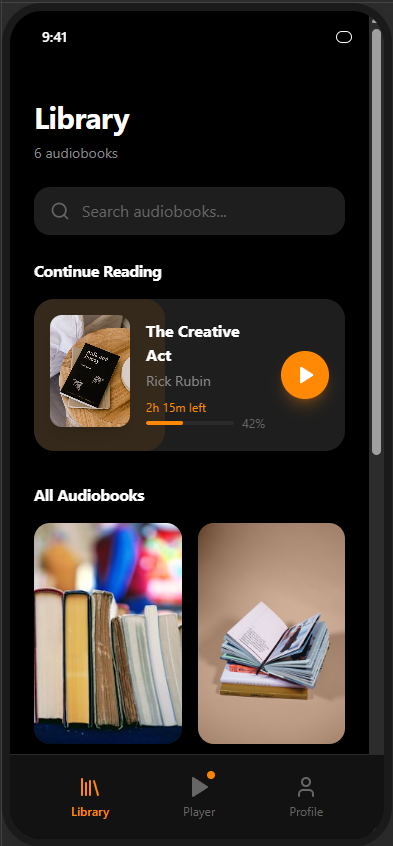
\includegraphics[width=0.35\textwidth]{./Figma pictures/HomeScreen - Library.png} &
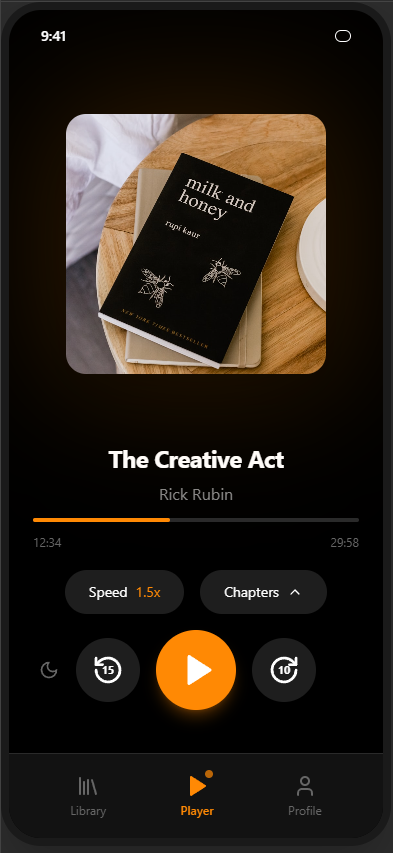
\includegraphics[width=0.35\textwidth]{./Figma pictures/Player Page.png} \\
\textbf{(a)} Library Screen & \textbf{(b)} Player Screen \\[0.5em]
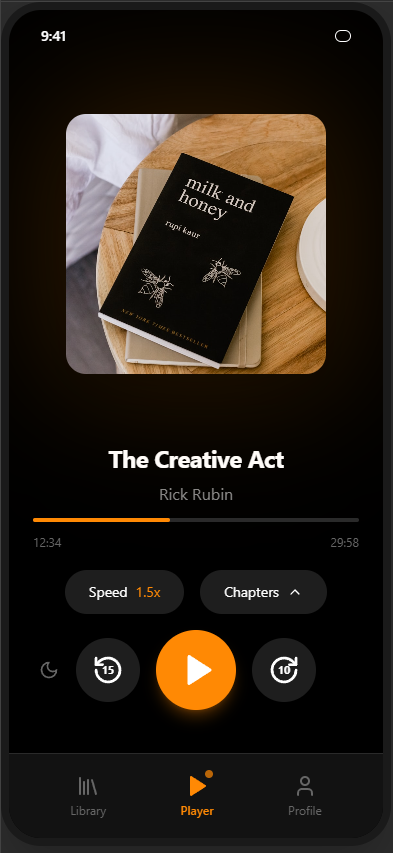
\includegraphics[width=0.35\textwidth]{./Figma pictures/Profile Page.png} &
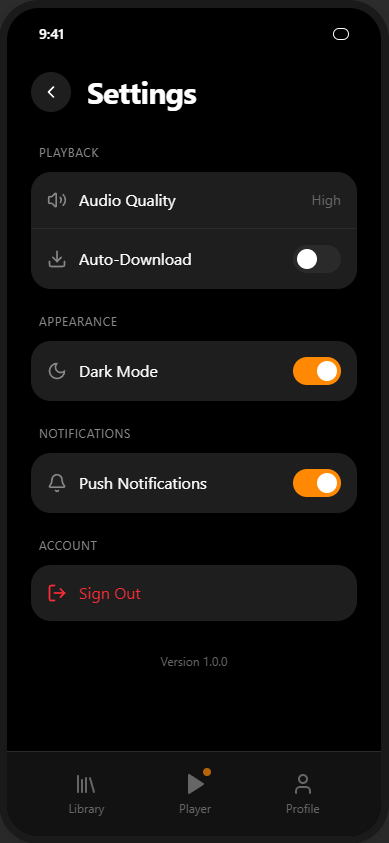
\includegraphics[width=0.35\textwidth]{./Figma pictures/Settings Page.png} \\
\textbf{(c)} Profile Screen & \textbf{(d)} Settings Screen
\end{tabular}
\caption{Main application screens showing library browsing, audio playback, user profile, and settings interfaces}
\end{figure}

\subsection{UI Flow Diagram}

\begin{figure}[H]
\centering
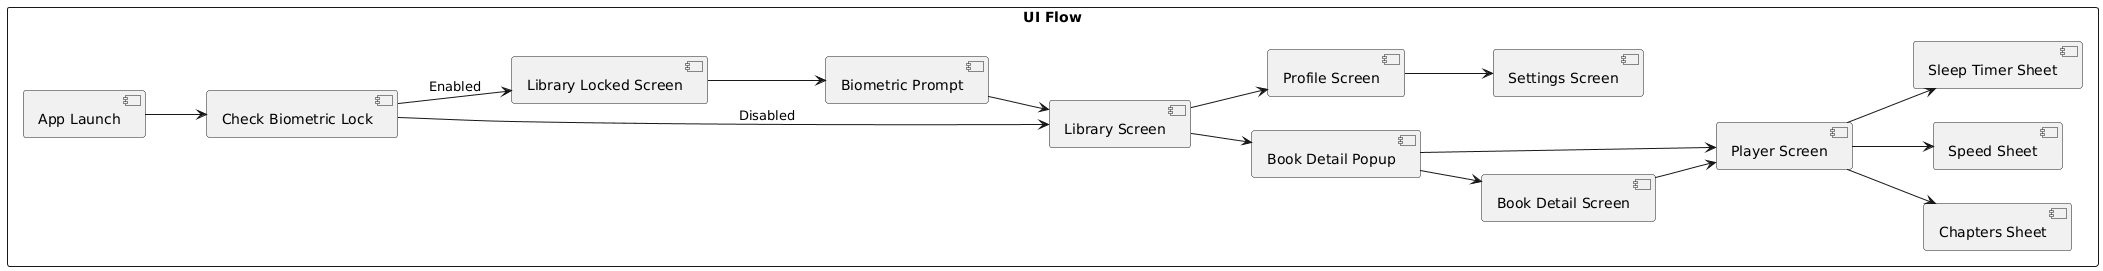
\includegraphics[width=0.9\textwidth]{./diagrams/exports/ui_flow.png}
\caption{UI Flow Diagram}
\end{figure}

The UI flow begins with app launch and biometric authentication check (if enabled). Users navigate from the library to book details and player screens, with access to settings and profile screens. The player screen provides access to chapters, playback speed, and sleep timer controls.

\subsection{Component Diagram}

\begin{figure}[H]
\centering
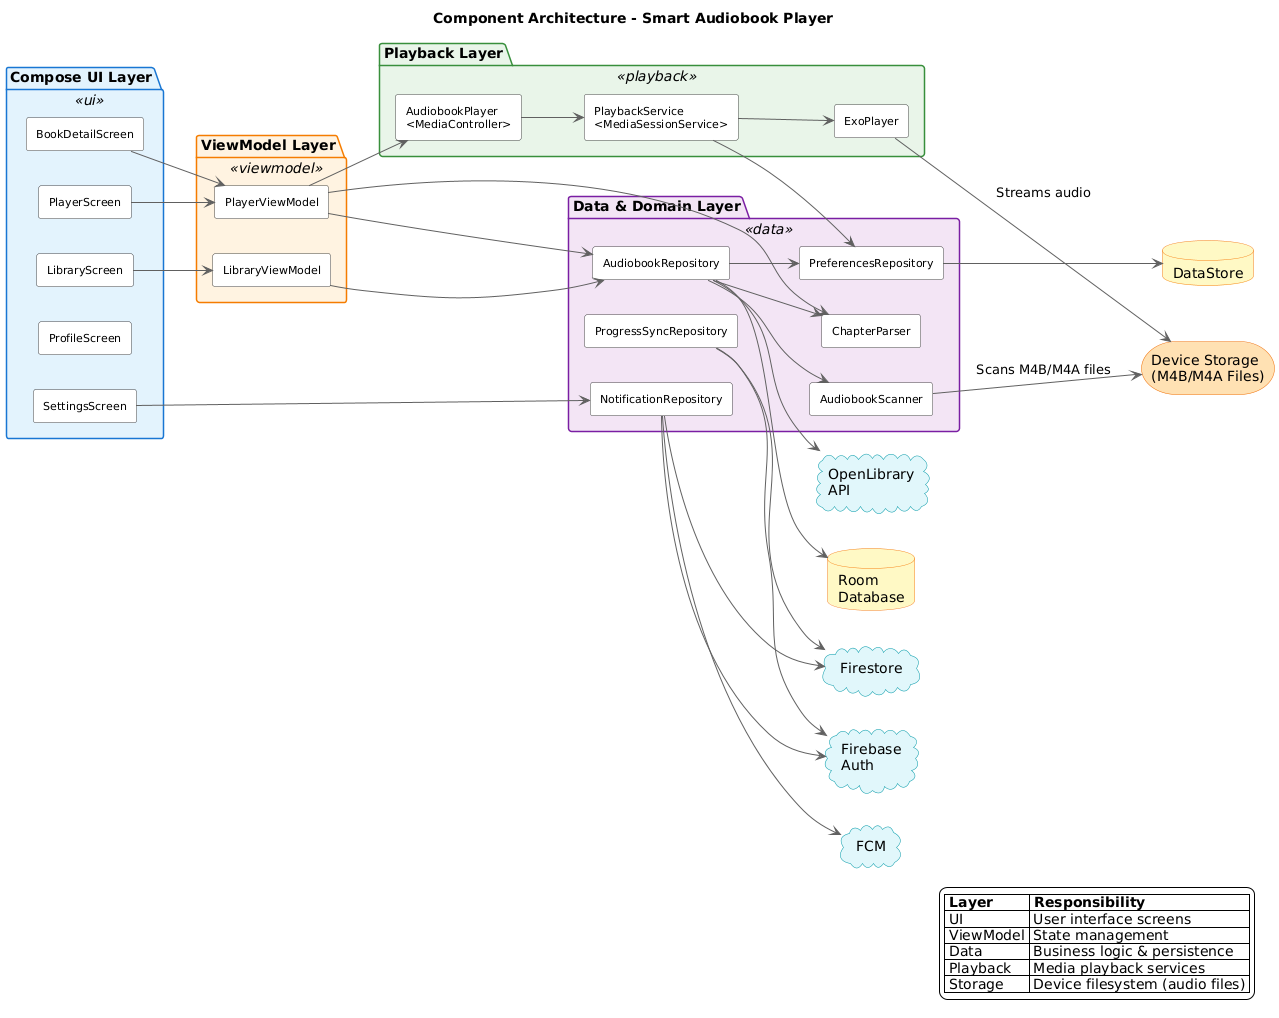
\includegraphics[width=0.95\textwidth]{./diagrams/exports/component_diagram.png}
\caption{Component Architecture Diagram}
\end{figure}

The architecture follows clean MVVM patterns with clear separation between UI layer (Compose screens), ViewModel layer, Data/Domain layer (repositories), Playback layer (Media3 components), local storage (Room/DataStore for metadata and preferences), and external services (Firebase, OpenLibrary API).

\textbf{Device Storage Integration:} The \texttt{AudiobookScanner} component scans the device filesystem to discover M4B/M4A audiobook files stored locally. \texttt{ExoPlayer} streams audio directly from these local file paths during playback. Only metadata and progress are persisted in Room database---the actual audio files remain in device storage and are never copied or moved.

\subsection{Use Case Diagram}

\begin{figure}[H]
\centering
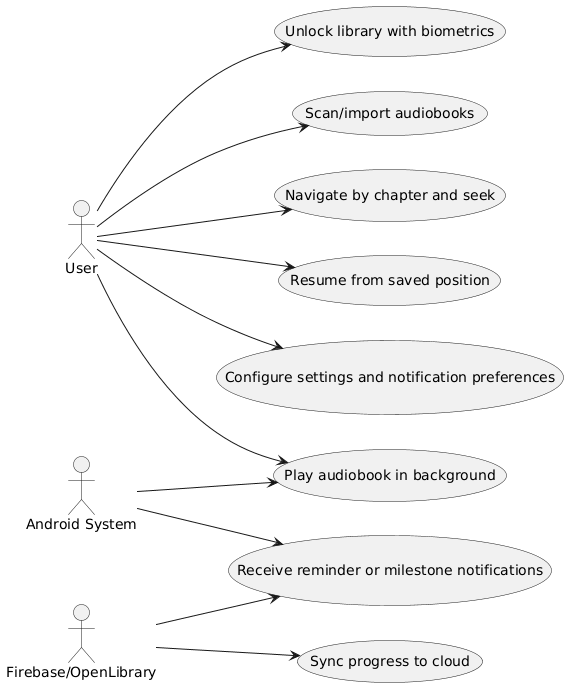
\includegraphics[width=0.9\textwidth]{./diagrams/exports/use_case_diagram.png}
\caption{Use Case Diagram}
\end{figure}

Key use cases include biometric authentication, audiobook scanning/import, background playback, chapter navigation, position resume, cloud progress sync, notification handling, and settings configuration. These involve interactions between the user, Android system, and cloud services.

\subsection{Sequence Diagram -- Audio Playback Flow}

\begin{figure}[H]
\centering
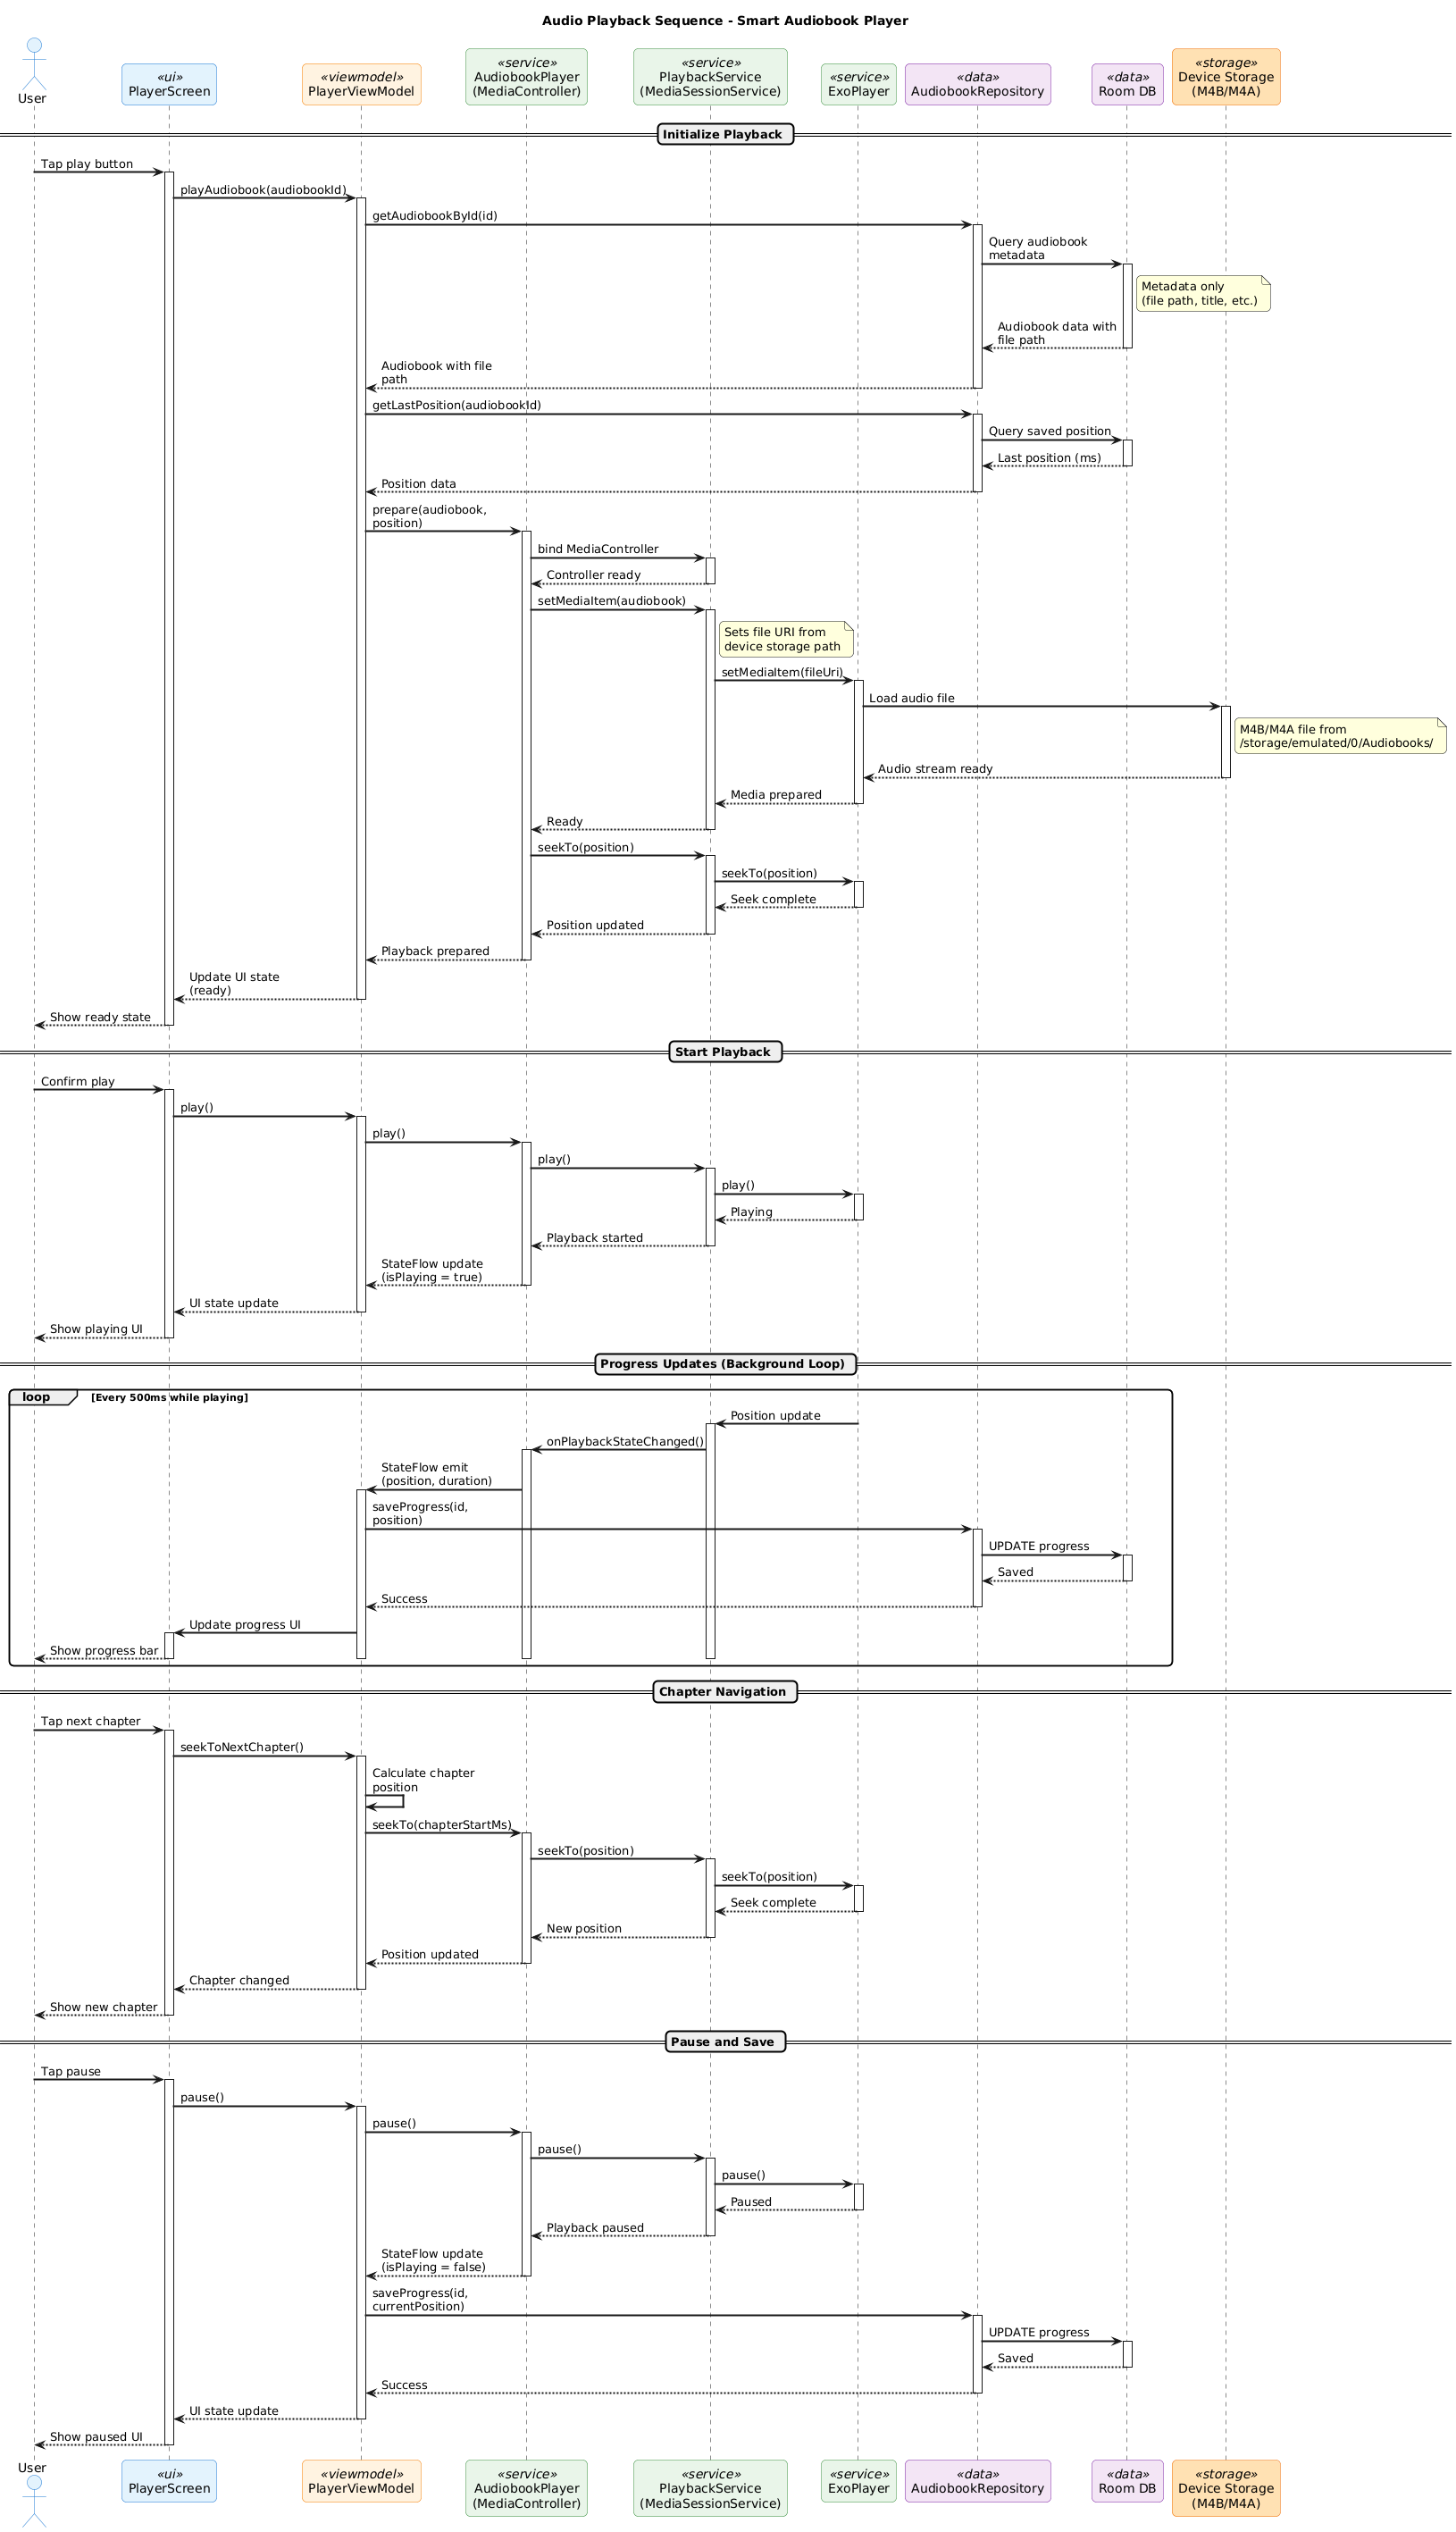
\includegraphics[width=0.75\textwidth]{./diagrams/exports/sequence_playback.png}
\caption{Audio Playback Sequence Diagram}
\end{figure}

The sequence diagram illustrates the complete audio playback lifecycle, capturing five key interaction phases:

\begin{enumerate}[noitemsep]
    \item \textbf{Initialization:} User taps play, triggering a chain that loads audiobook metadata (including local file path) and last saved position from Room database. The \texttt{Player-} \texttt{View-} \texttt{Model} coordinates retrieval through \texttt{Audiobook-} \texttt{Repository}. Note: Room stores only metadata; the actual M4B/M4A file remains in device storage.

    \item \textbf{Media preparation:} The \texttt{Audiobook-} \texttt{Player} (MediaController facade) binds to \texttt{Playback-} \texttt{Service} and configures the underlying \texttt{ExoPlayer} with the media item. ExoPlayer loads the audio file directly from the device filesystem using the local file URI.

    \item \textbf{Playback control:} User confirmation triggers play command down through the layers to ExoPlayer, which begins streaming audio from the local file. State updates flow back up through StateFlow emissions, keeping UI reactive.

    \item \textbf{Progress tracking:} A background loop runs every 500ms during playback, persisting current position to Room DB and syncing to Firestore. This enables accurate resume and cross-device continuity without affecting the source audio file.

    \item \textbf{Chapter navigation:} User-initiated chapter jumps calculate target position in \texttt{Player-} \texttt{View-} \texttt{Model}, issue seek commands to the playback service, and update UI with new chapter context. All chapter metadata is extracted from the M4B file itself during initial scanning.
\end{enumerate}

This design demonstrates clear separation of concerns: UI layer handles user interaction, ViewModel manages state and business logic, service layer handles media playback lifecycle and streams from device storage, and repository layer abstracts metadata persistence. The unidirectional data flow (actions down, state up) follows Android best practices for predictable state management.

\section{Testing and Validation}

\subsection{Test Content}

The application was tested with the following audiobook content:

\begin{itemize}[noitemsep]
    \item \textbf{Atomic Habits} by James Clear --- M4B format, approximately 5 hours 35 minutes, 28 chapters. Used as the primary test file for playback, chapter navigation, resume accuracy, and cloud sync validation.
    \item \textbf{Alice's Adventures in Wonderland} by Lewis Carroll --- M4B format sourced from \textbf{LibriVox} (\url{https://librivox.org}), a volunteer-driven project that provides free public domain audiobooks. LibriVox recordings are in the public domain and free to use for any purpose. This file was used to validate multi-book library behaviour and scanning.
\end{itemize}

\subsection{Test Scenarios Validated}

The following scenarios were verified on a Pixel 9 Pro XL emulator (API 35):

\begin{enumerate}[noitemsep]
    \item \textbf{Firebase Authentication:} Account creation (email/password), sign in, sign out, and session persistence across app restarts.
    \item \textbf{Playback lifecycle:} Play, pause, skip forward (30s), skip backward (15s), chapter seek, speed adjustment (0.5x--2.0x), and sleep timer (timed and end-of-chapter modes).
    \item \textbf{Background playback:} Audio continues when app is backgrounded. Media notification appears with playback controls. Notification controls (play/pause/skip) function correctly.
    \item \textbf{Resume accuracy:} After pausing and force-stopping the app, re-opening resumes from the exact saved position.
    \item \textbf{Firestore sync:} During playback, progress data (position, chapter, duration, book title, playback speed, per-chapter progress) is written to Firestore under \texttt{users/\{uid\}/progress/\{bookId\}}. Verified via Firebase Console that all fields are populated correctly.
    \item \textbf{Library scanning:} App correctly discovers and indexes M4B files from the device's Audiobooks directory, extracting metadata (title, author, duration, cover art) and chapter information.
    \item \textbf{Biometric lock:} When enabled in Settings, the lock screen appears on app launch and requires biometric authentication.
    \item \textbf{Notification workflows:} Daily reminder scheduling, configurable reminder time, and per-category notification toggles (reminders, milestones, streaks).
\end{enumerate}

\subsection{Firebase Data Verification}

Firestore data was verified directly against the database after a test session. Example document at \texttt{users/\{uid\}/progress/850506232}:

\begin{lstlisting}
{
  "bookTitle": "Atomic Habits",
  "positionMs": 409246,
  "totalDurationMs": 20132443,
  "lastChapter": 2,
  "playbackSpeed": 1.0,
  "chapterProgress": "{\"1\":1,\"2\":0.407}",
  "lastUpdated": "2026-03-31T01:16:47.494Z"
}
\end{lstlisting}

The user document at \texttt{users/\{uid\}} stores the FCM token for push notification delivery:

\begin{lstlisting}
{
  "fcmToken": "<device_token>",
  "tokenUpdatedAt": 1774919745489
}
\end{lstlisting}

Firestore security rules enforce that authenticated users can only read and write their own documents:

\begin{lstlisting}
match /users/{userId} {
  allow read, write: if request.auth != null
                     && request.auth.uid == userId;
  match /progress/{bookId} {
    allow read, write: if request.auth != null
                       && request.auth.uid == userId;
  }
}
\end{lstlisting}

\section{Conclusion}

Smart Audiobook Player delivers a complete end-to-end Android audiobook experience that aligns with the course goals and the original synopsis direction. The project demonstrates practical use of modern Android architecture and media APIs, especially through the Media3 \texttt{Media-} \texttt{Session-} \texttt{Service} approach, chapter-aware playback logic, and a Compose-first UI implementation.

From a technical perspective, the main achievement is the playback architecture: decoupling UI from media service via \texttt{MediaController}/\texttt{MediaSession}, preserving playback continuity across app state changes, and supporting audiobook-specific controls such as 15s/30s skip, chapter navigation, speed control, and sleep timer. The implementation also shows effective persistence strategy through Room and DataStore for local state, combined with Firestore for cross-device continuity.

All twelve requirements from the specification have been implemented and verified. Firebase Authentication and Firestore sync are fully operational with proper security rules. The notification system supports daily reminders, listening streaks, and book completion milestones. Biometric library lock is user-configurable via the Settings screen.

The most important insights gained during development were:
\begin{itemize}[noitemsep]
    \item Media containers are inconsistent in chapter metadata encoding, so robust fallback parsing is essential for M4B compatibility across different encoder tools.
    \item Long-form audio apps need frequent but controlled persistence updates to balance resume accuracy against battery and I/O cost---500ms debounced writes proved to be an effective trade-off.
    \item Cloud sync must be integrated directly into the playback lifecycle (not treated as a separate concern) to ensure data reaches Firestore reliably and with complete field coverage.
    \item Firestore security rules are critical infrastructure, not an afterthought---they must match the exact document path structure used by the application code.
\end{itemize}

\section{Known Bugs and Issues}

{\footnotesize
\begin{longtable}{|p{0.6cm}|>{\RaggedRight}p{4cm}|>{\RaggedRight}p{2.2cm}|>{\RaggedRight}p{2.8cm}|>{\RaggedRight}p{3cm}|}
\hline
\textbf{ID} & \textbf{Issue} & \textbf{Impact} & \textbf{Current Evidence} & \textbf{Suggested Next Step} \\ \hline
\endfirsthead
\hline
\textbf{ID} & \textbf{Issue} & \textbf{Impact} & \textbf{Current Evidence} & \textbf{Suggested Next Step} \\ \hline
\endhead
K1 & Notification icons use default system icon & Minor visual inconsistency & Uses generic Android icon & Update with custom app icon \\ \hline
K2 & Chapter display formatting varies on small screens & Minor text overflow & Long chapter names may clip & Add ellipsis or adaptive wrapping \\ \hline
K3 & Loading indicators use standard Material style & Minor UX polish & Default \texttt{Circular-} \texttt{Progress-} \texttt{Indicator} used & Consider custom branded animations \\ \hline
K4 & Error messages surface technical details & UX clarity & Raw exception text shown on some failures & Replace with user-friendly messages \\ \hline
K5 & Automated test suite not yet present & Regression risk & Test dependencies configured but no test files & Add unit tests for ViewModels and repositories \\ \hline
K6 & Some notification error paths silently catch exceptions & Reduced observability & Silent \texttt{catch} blocks in notification services & Add structured logging and retry logic \\ \hline
\end{longtable}
}

\end{document}
